\subsection{Sample Memory} \label{subsec:Sample_Memory} 
The Sample Control module will have to store \SIQ{320}{\kilo\bit} of sample data from the ADC before the MCU starts reading them, as mentioned in section \refq{subsubsec:CommunicationDatarate}. The Artix 7 FPGA development\cite{CMOD_A7_AT35T} board being used comes with \SIQ{4}{\mega\bit} of external asynchronous SRAM from ISSI\cite{ISSISRAM} that will be used to store the sampled data. The memory is organized as an array of 512K x 8 bit values, and because the ADC data are 16 bit values the Sample Control module should have hardware to store each sample in two distinct memory addresses in the external memory.

The IS61 SRAM has the functional block diagram shown on figure \refq{fig:7_2_5_IS61Block}.

\begin{figure}[H]
    \centering
    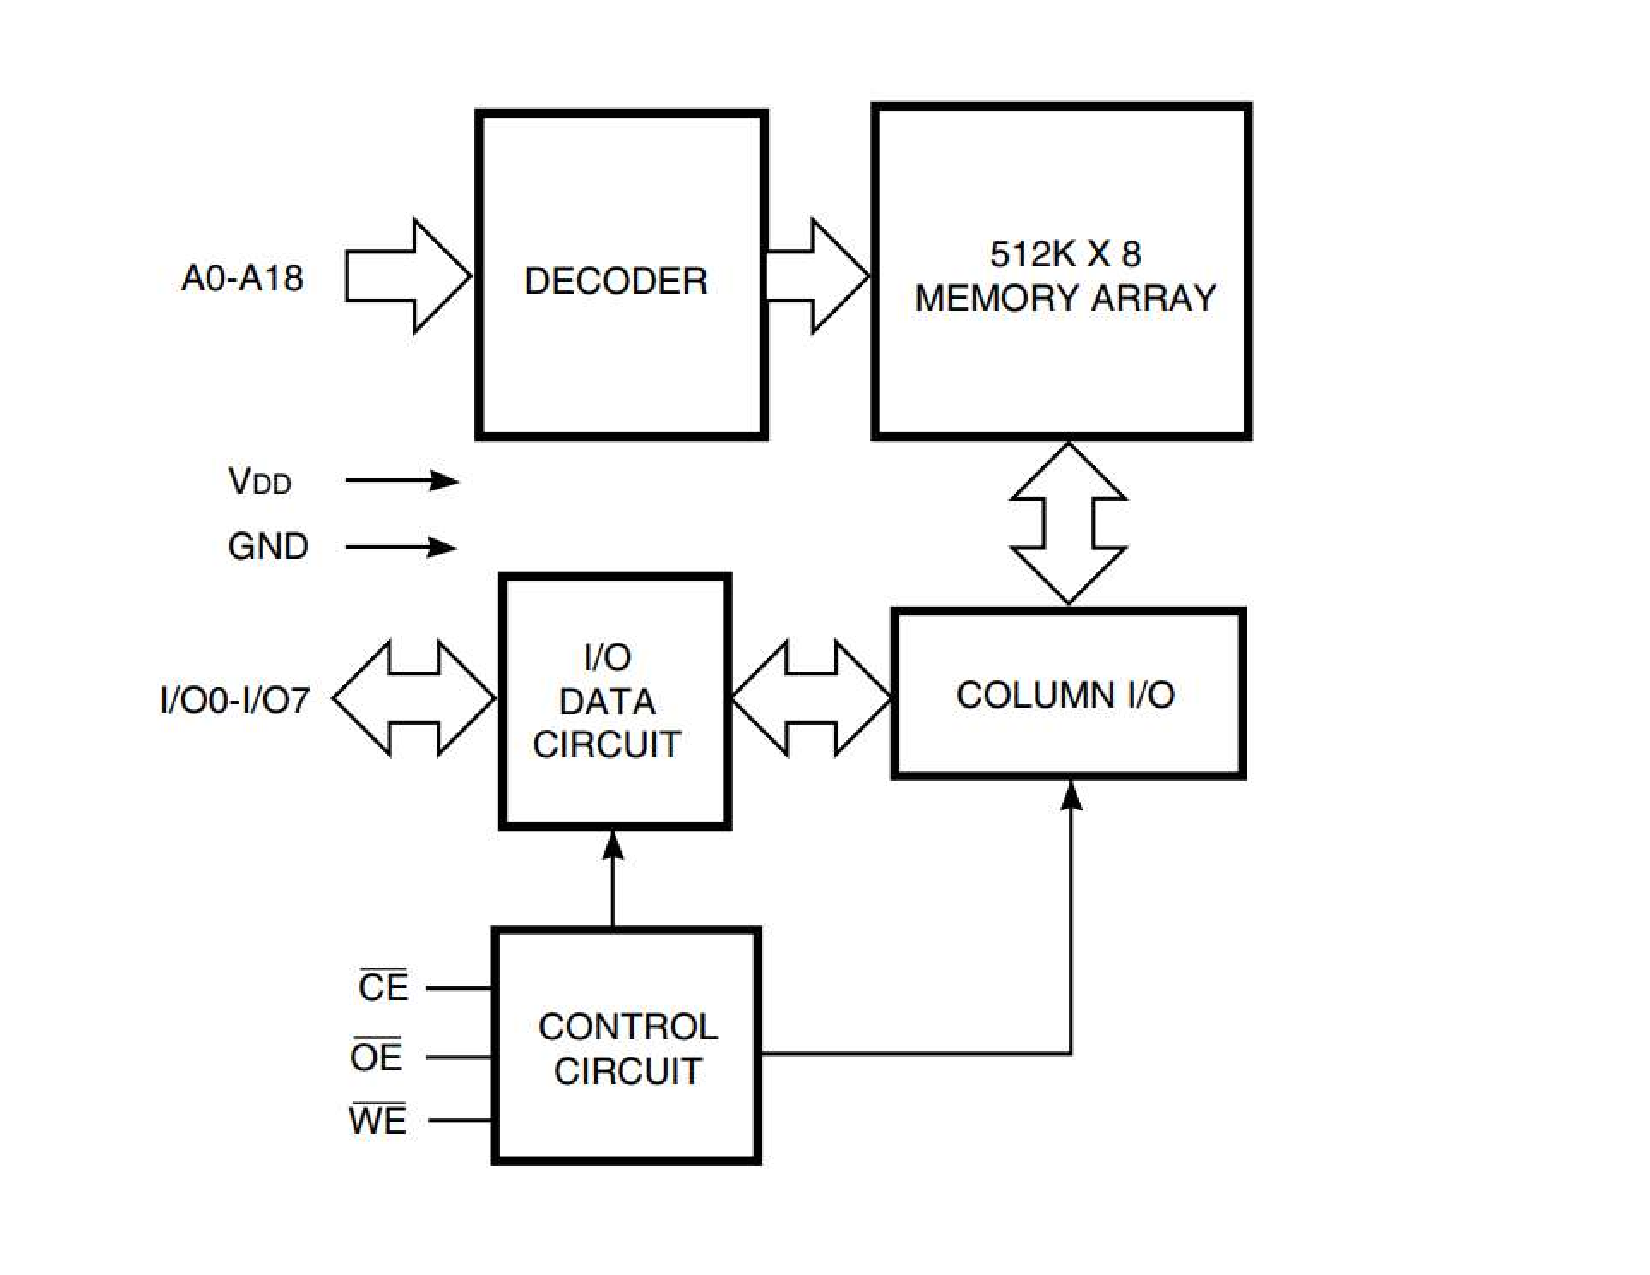
\includegraphics[clip, trim=0 0 0 0, width=0.65\textwidth]{Sections/7_SystemDesign/Figures/7_2_5_IS61_BLOCK_DIAGRAM.pdf}
    \caption{The functional block diagram for the IS61 SRAM\cite{ISSISRAM}. The SRAM uses a 19bit address bus, 8 bit bidirectional data bus along with 3 control signals.}
    \label{fig:7_2_5_IS61Block}
\end{figure}

The FPGA will have to control the address bus, data bus and control signals shown on figure \refq{fig:7_2_5_IS61Block} in order to write to, and read from, the IC. The control signals are Chip Enable (CE), Output Enable (OE) and Write Enable (WE) and they are all active-low signals. The CE input is used to put the the IC into a low-power standby mode, this is not used for this project, so CE is tied to logic '0' at all times. The OE signal controls the state of the output drivers on the chip and a '0' activates the outputs while a '1' sets them into a high impedance state. The WE input controls if a write or read is happening to/from the IC. Note how there is no clock signal, so the memory is asynchronous and any reads, or writes, happens when the WE signal changes state.

In order to write to RAM the FPGA should have hardware that follows the write cycle shown on figure \refq{fig:7_2_5_IS61_WRITE} from the IS61 datasheet.
\begin{figure}[H]
    \centering
    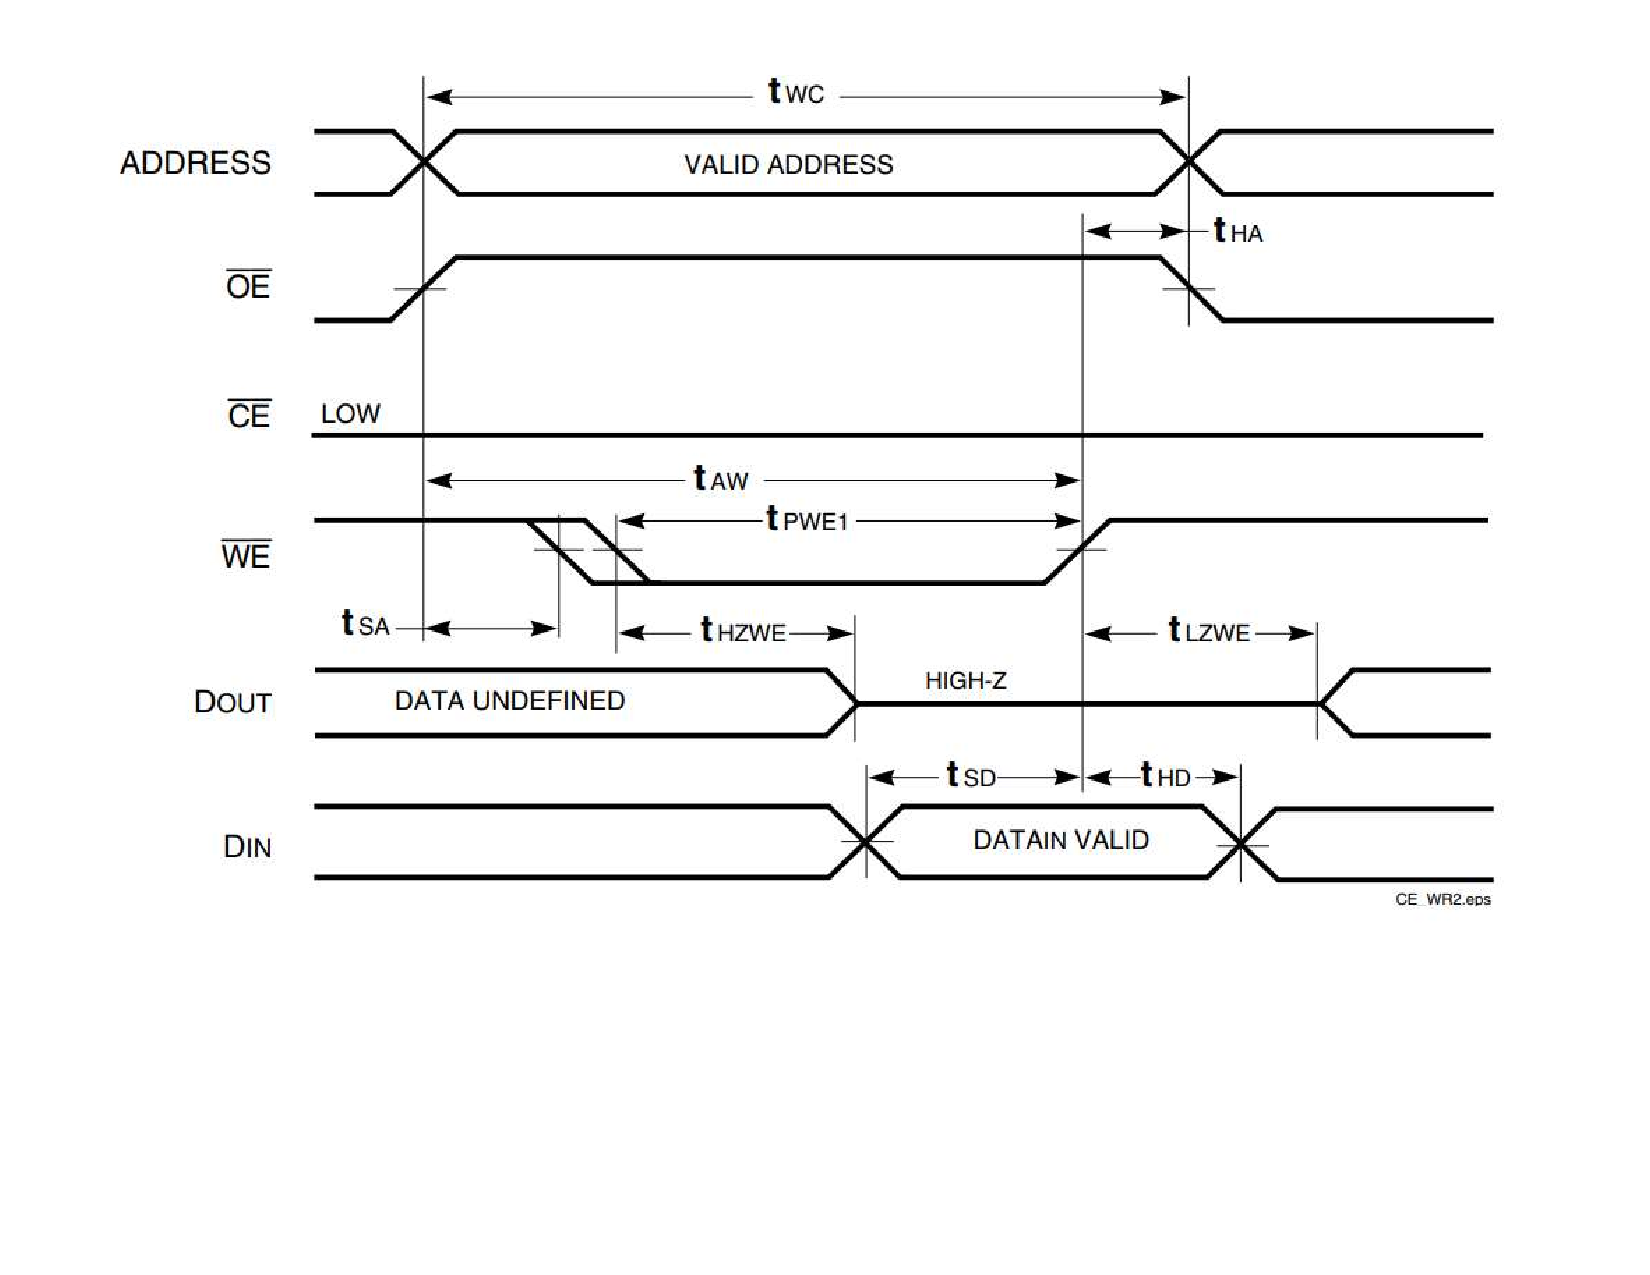
\includegraphics[clip, trim=0 150 0 0, width=0.8\textwidth]{Sections/7_SystemDesign/Figures/7_2_5_IS61_WriteCycle.pdf}
    \caption{A complete write cycle for the IS61 SRAM IC\cite{ISSISRAM}. In order to write to RAM the FPGA should go through the following sequence of events; Set Address to Address bus, Disable output drivers with OE = '1', assert Write Enable with WE = '0', set data to data bus and finish the sequence with WE = '1' to CLK the data byte into RAM.}
    \label{fig:7_2_5_IS61_WRITE}
\end{figure}

The write sequence shown on figure \refq{fig:7_2_5_IS61_WRITE} has been implemented in hardware as a state machine as shown in the code listing list \refq{lst:7_2_5_Write_FSM}.
\lstinputlisting[language=C ,style = c,firstnumber=1, linerange=84-102, caption={VHDL code for the write sequence state machine}, label={lst:7_2_5_Write_FSM}]{Sections/7_SystemDesign/Code/ext_mem_read_write.vhd}

The state machine will go through steps 1 to 4 and transition on every rising edge of a CLK signal. As shown on figure \refq{fig:7_2_5_IS61_WRITE} the FSM will, in step 1, start by disabling the output drivers with OE = '1' and setting the address unto the address bus. In step 2 it asserts the WE signal. In step 3 it sets 1 byte of the sample data unto the data bus and it step 4 it releases WE and thus CLKs the data into RAM and returns to the initial state, ready for the next write.

Note how on figure \refq{fig:7_2_5_IS61_WRITE} there is a significant amount of timings that the hardware must obey in order for the IC to function properly. It was found during testing that by making a simple FSM as shown in listing \refq{lst:7_2_5_Write_FSM}, with the 4 steps mentioned in the captions of figure \refq{fig:7_2_5_IS61_WRITE}, it was possible to get \SIQ{12}{\mega\bit}/s data rates without corruption of data. Data gets corrupted when the state machines clock input exceed \SIQ{15}{\mega\hertz}. A data rate of \SIQ{12}{\mega\bit}/s exceeds the expected data from the ADC module and is sufficient for the task, so no further work is required for the memory in this case.

A read from the IS61 SRAM follows a similar procedure as shown on the read cycle timing diagram on figure \refq{fig:7_2_5_IS61_READ}.
\begin{figure}[H]
    \centering
    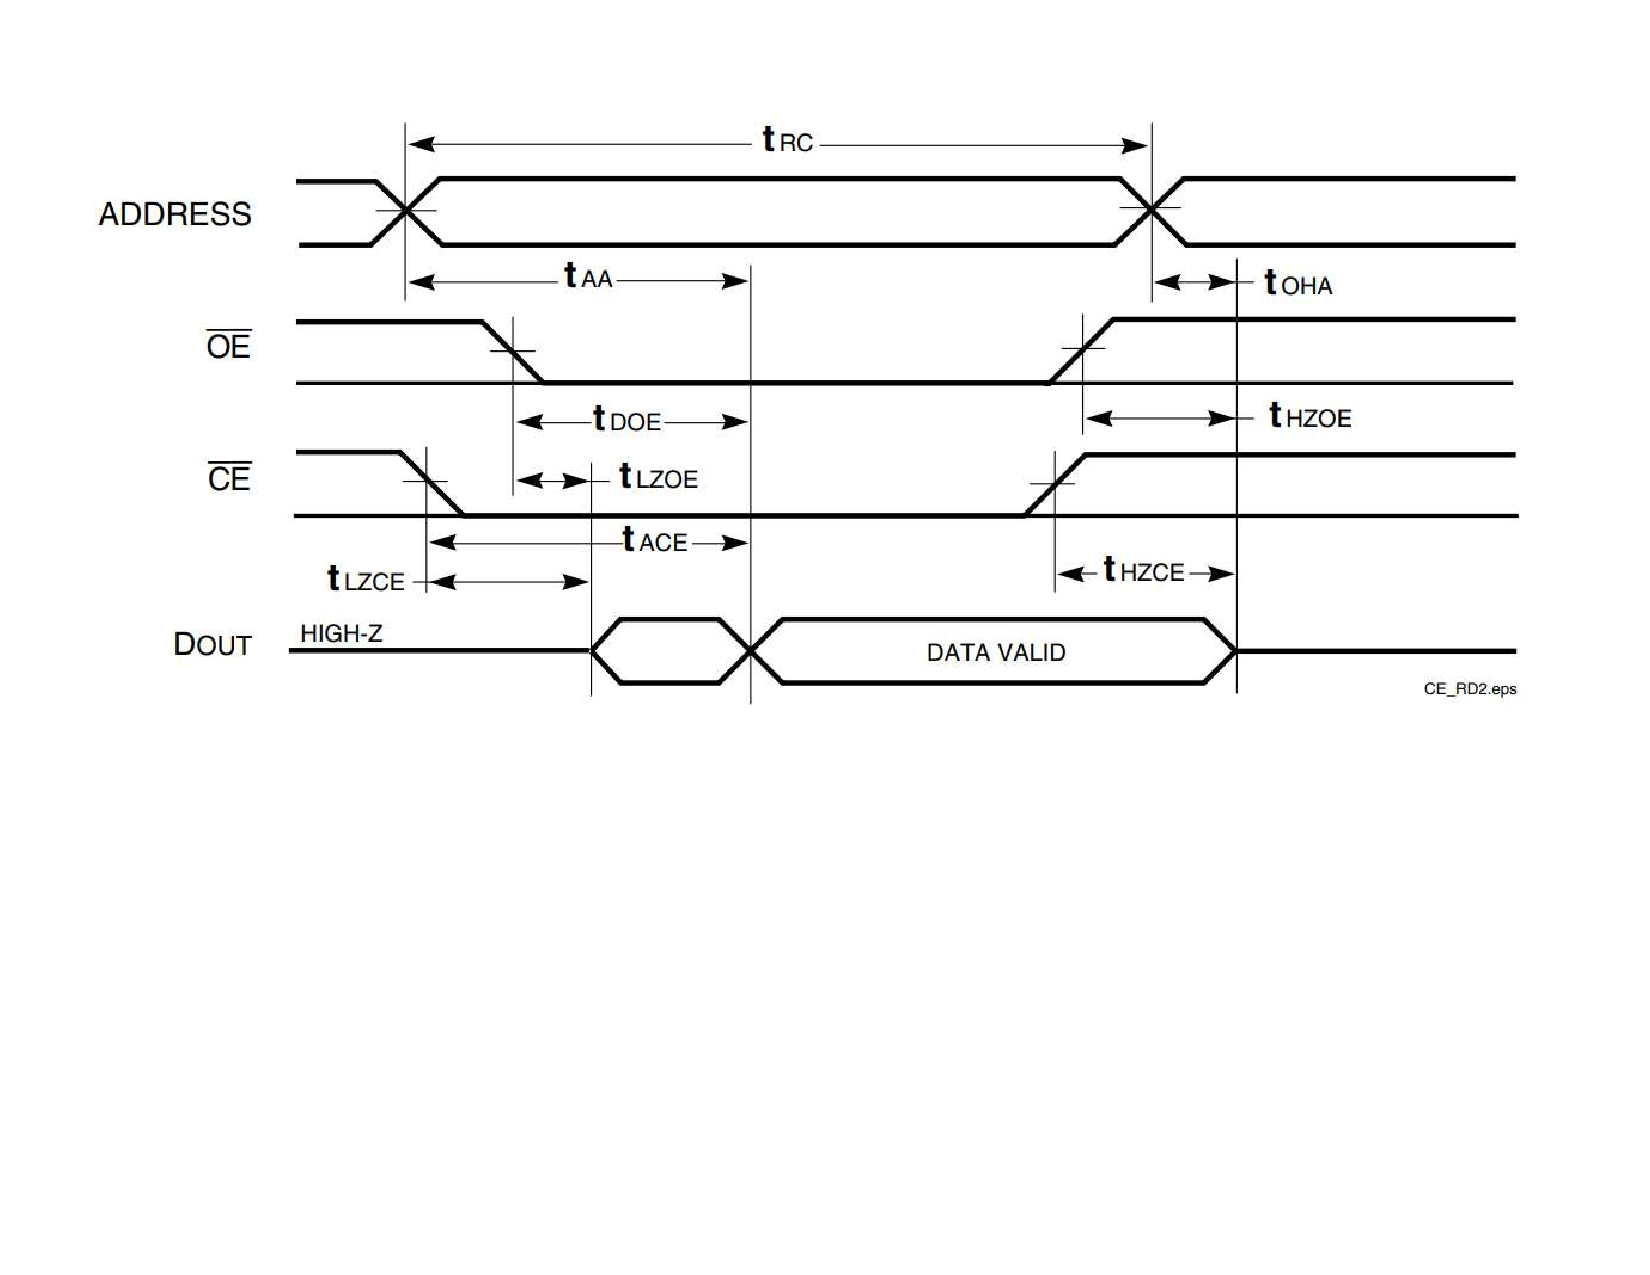
\includegraphics[clip, trim=0 250 0 0, width=0.8\textwidth]{Sections/7_SystemDesign/Figures/7_2_5_IS61_ReadCycle.pdf}
    \caption{A complete read cycle for the IS61 SRAM IC\cite{ISSISRAM}. An address must be set to the address bus, when an address is set the output drivers are enable with OE = '0'. Data is available on the data bus when OE transitions back to OE = '1'. CE is not being controlled in this projects application and is tied to logic '0'.}
    \label{fig:7_2_5_IS61_READ}
\end{figure}

Note how on figure \refq{fig:7_2_5_IS61_READ} the WE signal is not displayed, but WE should be held high for a read cycle in order to work properly. The CE signal is, also, not being controlled in this project and is still tied to '0'. The read cycle is also being controlled by a state machine and the code listing for this can be seen on listing \refq{lst:7_2_5_READ_FSM}.

\lstinputlisting[language=C ,style = c,firstnumber=1, linerange=130-154, caption={VHDL code for the read sequence state machine}, label={lst:7_2_5_READ_FSM}]{Sections/7_SystemDesign/Code/ext_mem_read_write.vhd} 

The FSM shown in listing \refq{lst:7_2_5_READ_FSM} steps through the read cycle shown on figure \refq{fig:7_2_5_IS61_READ}. It enables read mode by setting WE = '1' and putting an address on the address bus. Next, the output drivers are enabled. In step 3 a single CLK is skipped because this was found to greatly increase the reliablity of reads during testing as the IC required more time to setup the data on the bus. Again, the amount of work being done to ensure the correct timing is minimal, but this was sufficient for \SIQ{12}{\mega\bit}/s data rates. In step 4 the data is transfered to the FPGA and the output drivers are disabled again.

If the project had more time for development it would be possible to increase the data rates of this communication bus by paying greater attention to the timings of the IS61 SRAM IC.